% Options for packages loaded elsewhere
\PassOptionsToPackage{unicode}{hyperref}
\PassOptionsToPackage{hyphens}{url}
\PassOptionsToPackage{dvipsnames,svgnames,x11names}{xcolor}
%
\documentclass[
  letterpaper,
  DIV=11,
  numbers=noendperiod]{scrartcl}

\usepackage{amsmath,amssymb}
\usepackage{iftex}
\ifPDFTeX
  \usepackage[T1]{fontenc}
  \usepackage[utf8]{inputenc}
  \usepackage{textcomp} % provide euro and other symbols
\else % if luatex or xetex
  \usepackage{unicode-math}
  \defaultfontfeatures{Scale=MatchLowercase}
  \defaultfontfeatures[\rmfamily]{Ligatures=TeX,Scale=1}
\fi
\usepackage{lmodern}
\ifPDFTeX\else  
    % xetex/luatex font selection
\fi
% Use upquote if available, for straight quotes in verbatim environments
\IfFileExists{upquote.sty}{\usepackage{upquote}}{}
\IfFileExists{microtype.sty}{% use microtype if available
  \usepackage[]{microtype}
  \UseMicrotypeSet[protrusion]{basicmath} % disable protrusion for tt fonts
}{}
\makeatletter
\@ifundefined{KOMAClassName}{% if non-KOMA class
  \IfFileExists{parskip.sty}{%
    \usepackage{parskip}
  }{% else
    \setlength{\parindent}{0pt}
    \setlength{\parskip}{6pt plus 2pt minus 1pt}}
}{% if KOMA class
  \KOMAoptions{parskip=half}}
\makeatother
\usepackage{xcolor}
\setlength{\emergencystretch}{3em} % prevent overfull lines
\setcounter{secnumdepth}{-\maxdimen} % remove section numbering
% Make \paragraph and \subparagraph free-standing
\makeatletter
\ifx\paragraph\undefined\else
  \let\oldparagraph\paragraph
  \renewcommand{\paragraph}{
    \@ifstar
      \xxxParagraphStar
      \xxxParagraphNoStar
  }
  \newcommand{\xxxParagraphStar}[1]{\oldparagraph*{#1}\mbox{}}
  \newcommand{\xxxParagraphNoStar}[1]{\oldparagraph{#1}\mbox{}}
\fi
\ifx\subparagraph\undefined\else
  \let\oldsubparagraph\subparagraph
  \renewcommand{\subparagraph}{
    \@ifstar
      \xxxSubParagraphStar
      \xxxSubParagraphNoStar
  }
  \newcommand{\xxxSubParagraphStar}[1]{\oldsubparagraph*{#1}\mbox{}}
  \newcommand{\xxxSubParagraphNoStar}[1]{\oldsubparagraph{#1}\mbox{}}
\fi
\makeatother

\usepackage{color}
\usepackage{fancyvrb}
\newcommand{\VerbBar}{|}
\newcommand{\VERB}{\Verb[commandchars=\\\{\}]}
\DefineVerbatimEnvironment{Highlighting}{Verbatim}{commandchars=\\\{\}}
% Add ',fontsize=\small' for more characters per line
\usepackage{framed}
\definecolor{shadecolor}{RGB}{241,243,245}
\newenvironment{Shaded}{\begin{snugshade}}{\end{snugshade}}
\newcommand{\AlertTok}[1]{\textcolor[rgb]{0.68,0.00,0.00}{#1}}
\newcommand{\AnnotationTok}[1]{\textcolor[rgb]{0.37,0.37,0.37}{#1}}
\newcommand{\AttributeTok}[1]{\textcolor[rgb]{0.40,0.45,0.13}{#1}}
\newcommand{\BaseNTok}[1]{\textcolor[rgb]{0.68,0.00,0.00}{#1}}
\newcommand{\BuiltInTok}[1]{\textcolor[rgb]{0.00,0.23,0.31}{#1}}
\newcommand{\CharTok}[1]{\textcolor[rgb]{0.13,0.47,0.30}{#1}}
\newcommand{\CommentTok}[1]{\textcolor[rgb]{0.37,0.37,0.37}{#1}}
\newcommand{\CommentVarTok}[1]{\textcolor[rgb]{0.37,0.37,0.37}{\textit{#1}}}
\newcommand{\ConstantTok}[1]{\textcolor[rgb]{0.56,0.35,0.01}{#1}}
\newcommand{\ControlFlowTok}[1]{\textcolor[rgb]{0.00,0.23,0.31}{\textbf{#1}}}
\newcommand{\DataTypeTok}[1]{\textcolor[rgb]{0.68,0.00,0.00}{#1}}
\newcommand{\DecValTok}[1]{\textcolor[rgb]{0.68,0.00,0.00}{#1}}
\newcommand{\DocumentationTok}[1]{\textcolor[rgb]{0.37,0.37,0.37}{\textit{#1}}}
\newcommand{\ErrorTok}[1]{\textcolor[rgb]{0.68,0.00,0.00}{#1}}
\newcommand{\ExtensionTok}[1]{\textcolor[rgb]{0.00,0.23,0.31}{#1}}
\newcommand{\FloatTok}[1]{\textcolor[rgb]{0.68,0.00,0.00}{#1}}
\newcommand{\FunctionTok}[1]{\textcolor[rgb]{0.28,0.35,0.67}{#1}}
\newcommand{\ImportTok}[1]{\textcolor[rgb]{0.00,0.46,0.62}{#1}}
\newcommand{\InformationTok}[1]{\textcolor[rgb]{0.37,0.37,0.37}{#1}}
\newcommand{\KeywordTok}[1]{\textcolor[rgb]{0.00,0.23,0.31}{\textbf{#1}}}
\newcommand{\NormalTok}[1]{\textcolor[rgb]{0.00,0.23,0.31}{#1}}
\newcommand{\OperatorTok}[1]{\textcolor[rgb]{0.37,0.37,0.37}{#1}}
\newcommand{\OtherTok}[1]{\textcolor[rgb]{0.00,0.23,0.31}{#1}}
\newcommand{\PreprocessorTok}[1]{\textcolor[rgb]{0.68,0.00,0.00}{#1}}
\newcommand{\RegionMarkerTok}[1]{\textcolor[rgb]{0.00,0.23,0.31}{#1}}
\newcommand{\SpecialCharTok}[1]{\textcolor[rgb]{0.37,0.37,0.37}{#1}}
\newcommand{\SpecialStringTok}[1]{\textcolor[rgb]{0.13,0.47,0.30}{#1}}
\newcommand{\StringTok}[1]{\textcolor[rgb]{0.13,0.47,0.30}{#1}}
\newcommand{\VariableTok}[1]{\textcolor[rgb]{0.07,0.07,0.07}{#1}}
\newcommand{\VerbatimStringTok}[1]{\textcolor[rgb]{0.13,0.47,0.30}{#1}}
\newcommand{\WarningTok}[1]{\textcolor[rgb]{0.37,0.37,0.37}{\textit{#1}}}

\providecommand{\tightlist}{%
  \setlength{\itemsep}{0pt}\setlength{\parskip}{0pt}}\usepackage{longtable,booktabs,array}
\usepackage{calc} % for calculating minipage widths
% Correct order of tables after \paragraph or \subparagraph
\usepackage{etoolbox}
\makeatletter
\patchcmd\longtable{\par}{\if@noskipsec\mbox{}\fi\par}{}{}
\makeatother
% Allow footnotes in longtable head/foot
\IfFileExists{footnotehyper.sty}{\usepackage{footnotehyper}}{\usepackage{footnote}}
\makesavenoteenv{longtable}
\usepackage{graphicx}
\makeatletter
\def\maxwidth{\ifdim\Gin@nat@width>\linewidth\linewidth\else\Gin@nat@width\fi}
\def\maxheight{\ifdim\Gin@nat@height>\textheight\textheight\else\Gin@nat@height\fi}
\makeatother
% Scale images if necessary, so that they will not overflow the page
% margins by default, and it is still possible to overwrite the defaults
% using explicit options in \includegraphics[width, height, ...]{}
\setkeys{Gin}{width=\maxwidth,height=\maxheight,keepaspectratio}
% Set default figure placement to htbp
\makeatletter
\def\fps@figure{htbp}
\makeatother

\usepackage{fvextra}
\DefineVerbatimEnvironment{Highlighting}{Verbatim}{breaklines,commandchars=\\\{\}}
\DefineVerbatimEnvironment{OutputCode}{Verbatim}{breaklines,commandchars=\\\{\}}
\KOMAoption{captions}{tableheading}
\makeatletter
\@ifpackageloaded{caption}{}{\usepackage{caption}}
\AtBeginDocument{%
\ifdefined\contentsname
  \renewcommand*\contentsname{Table of contents}
\else
  \newcommand\contentsname{Table of contents}
\fi
\ifdefined\listfigurename
  \renewcommand*\listfigurename{List of Figures}
\else
  \newcommand\listfigurename{List of Figures}
\fi
\ifdefined\listtablename
  \renewcommand*\listtablename{List of Tables}
\else
  \newcommand\listtablename{List of Tables}
\fi
\ifdefined\figurename
  \renewcommand*\figurename{Figure}
\else
  \newcommand\figurename{Figure}
\fi
\ifdefined\tablename
  \renewcommand*\tablename{Table}
\else
  \newcommand\tablename{Table}
\fi
}
\@ifpackageloaded{float}{}{\usepackage{float}}
\floatstyle{ruled}
\@ifundefined{c@chapter}{\newfloat{codelisting}{h}{lop}}{\newfloat{codelisting}{h}{lop}[chapter]}
\floatname{codelisting}{Listing}
\newcommand*\listoflistings{\listof{codelisting}{List of Listings}}
\makeatother
\makeatletter
\makeatother
\makeatletter
\@ifpackageloaded{caption}{}{\usepackage{caption}}
\@ifpackageloaded{subcaption}{}{\usepackage{subcaption}}
\makeatother

\ifLuaTeX
  \usepackage{selnolig}  % disable illegal ligatures
\fi
\usepackage{bookmark}

\IfFileExists{xurl.sty}{\usepackage{xurl}}{} % add URL line breaks if available
\urlstyle{same} % disable monospaced font for URLs
\hypersetup{
  pdftitle={HW 1},
  pdfauthor={Bryan Mui - UID 506021334 - 14 April 2025},
  colorlinks=true,
  linkcolor={blue},
  filecolor={Maroon},
  citecolor={Blue},
  urlcolor={Blue},
  pdfcreator={LaTeX via pandoc}}


\title{HW 1}
\author{Bryan Mui - UID 506021334 - 14 April 2025}
\date{}

\begin{document}
\maketitle


\section{Problem 1}\label{problem-1}

\subsection{Part a}\label{part-a}

Find the theoretical min for the function: \[
f(x) = x^4 + 2x^2 + 1
\]

Solution: find f'(x) and f'\,`(x), set f'(x) to 0 and solve, and
f'\,'(x) needs to be \textgreater{} 0 to be a min

Step 1: find f'(x) and f'\,'(x) \begin{align}
  f(x) &= x^4 + 2x^2 + 1 \\ 
 f'(x) &= 4x^3 + 4x  \\
f''(x) &= 12x^2 + 4 \\
\end {align}

Step 2: set f'(x) to 0 and solve

\begin{align}
f'(x) &= 4x^3 + 4x  \\
    0 &= 4x^3 + 4x \\
    0 &= 4x(x^2 + 4)
\end{align}

We get \[x = 0\] and \[0 = x^2 +4\] which has no real solution

Step 3: check that f'\,'(x) needs to be \textgreater{} 0 to be a min

Our critical point is x = 0,

\begin{align}
f''(0)  &= 12(0)^2 + 4 \\
        &= 4
\end{align}

Since f'(x) = 0 at 0 and f'\,'(x) \textgreater{} 0 at that point,
\textbf{we have a min at x = 0, and plugging into f(0) we get the
minimum point}

\begin{center} (0, 1) \end{center}

\subsection{Part b}\label{part-b}

\subsubsection{0)}\label{section}

Use the gradient descent algorithm with \textbf{constant step size} and
with \textbf{back-tracking line search} to calculate \(x_{min}\)

\textbf{Constant step size descent is implemented as follows:}

\begin{enumerate}
\def\labelenumi{\arabic{enumi}.}
\tightlist
\item
  Select a random starting point \(x_0\)\\
\item
  While stopping criteria \textless{} tolerance, do:
\end{enumerate}

\begin{itemize}
\tightlist
\item
  Select \(η_k\)(as a constant)\\
\item
  Calculate \(x_{(k+1)} = x_k - η_k * ∇(f(x_k))\)\\
\item
  Calculate the value of stopping criterion
\end{itemize}

Stopping criteria: Stop if \(∣|∇(f(x_k)||_2 ≤ ϵ\)

\begin{Shaded}
\begin{Highlighting}[]
\CommentTok{\# Gradient descent algorithm that uses backtracking to minimize an objective function}

\NormalTok{gradient\_descent\_constant\_step }\OtherTok{\textless{}{-}} \ControlFlowTok{function}\NormalTok{(}\AttributeTok{tol =} \FloatTok{1e{-}6}\NormalTok{, }\AttributeTok{max\_iter =} \DecValTok{10000}\NormalTok{, }\AttributeTok{step\_size =} \FloatTok{0.01}\NormalTok{) \{}
  \CommentTok{\# Step 1: Initialize and select a random stopping point}
  \CommentTok{\# Initialize}
  \FunctionTok{set.seed}\NormalTok{(}\DecValTok{777}\NormalTok{) }\CommentTok{\# example seeding }
\NormalTok{  last\_iter }\OtherTok{\textless{}{-}} \DecValTok{0} \CommentTok{\# the last iteration ran}
\NormalTok{  eta }\OtherTok{\textless{}{-}}\NormalTok{ step\_size }\CommentTok{\# step size that is decided manually }
\NormalTok{  max\_iter }\OtherTok{\textless{}{-}}\NormalTok{ max\_iter }\CommentTok{\# max iterations before terminating if mininum isn\textquotesingle{}t found}
\NormalTok{  tolerance }\OtherTok{\textless{}{-}}\NormalTok{ tol }\CommentTok{\# tolerance for the stoppign criteria }
\NormalTok{  obj\_values }\OtherTok{\textless{}{-}} \FunctionTok{numeric}\NormalTok{(max\_iter) }\CommentTok{\# Stores the value of f(x)}
\NormalTok{  eta\_values }\OtherTok{\textless{}{-}} \FunctionTok{numeric}\NormalTok{(max\_iter)  }\CommentTok{\# To store eta values used each iteration}
\NormalTok{  eta\_values[}\DecValTok{1}\NormalTok{] }\OtherTok{\textless{}{-}}\NormalTok{ step\_size}
\NormalTok{  betas }\OtherTok{\textless{}{-}} \FunctionTok{numeric}\NormalTok{(max\_iter) }\CommentTok{\# Stores the value of x guesses}
\NormalTok{  x0 }\OtherTok{\textless{}{-}} \FunctionTok{runif}\NormalTok{(}\DecValTok{1}\NormalTok{, }\AttributeTok{min=}\SpecialCharTok{{-}}\DecValTok{10}\NormalTok{, }\AttributeTok{max=}\DecValTok{10}\NormalTok{) }\CommentTok{\# our first guess is somewhere between {-}10{-}10}
  
  \CommentTok{\# Set the objective function to the function to be minimized }
  \CommentTok{\# Objective function: f(x)}
\NormalTok{  obj\_function }\OtherTok{\textless{}{-}} \ControlFlowTok{function}\NormalTok{(x) \{}
    \FunctionTok{return}\NormalTok{(x}\SpecialCharTok{\^{}}\DecValTok{4} \SpecialCharTok{+} \DecValTok{2}\SpecialCharTok{*}\NormalTok{(x}\SpecialCharTok{\^{}}\DecValTok{2}\NormalTok{) }\SpecialCharTok{+} \DecValTok{1}\NormalTok{) }
\NormalTok{  \}}
  
  \CommentTok{\# Gradient function: d/dx of f(x)}
\NormalTok{  gradient }\OtherTok{\textless{}{-}} \ControlFlowTok{function}\NormalTok{(x) \{}
    \FunctionTok{return}\NormalTok{(}\DecValTok{4}\SpecialCharTok{*}\NormalTok{x}\SpecialCharTok{\^{}}\DecValTok{3} \SpecialCharTok{+} \DecValTok{4}\SpecialCharTok{*}\NormalTok{x)}
\NormalTok{  \}}
  
  \CommentTok{\# Append the first guess to the obj\_values and betas vector}
\NormalTok{  betas[}\DecValTok{1}\NormalTok{] }\OtherTok{\textless{}{-}}\NormalTok{ x0}
\NormalTok{  obj\_values[}\DecValTok{1}\NormalTok{] }\OtherTok{\textless{}{-}} \FunctionTok{obj\_function}\NormalTok{(x0)}
  
  \CommentTok{\# Step 2: While stopping criteria \textless{} tolerance, do:}
  \ControlFlowTok{for}\NormalTok{ (iter }\ControlFlowTok{in} \DecValTok{1}\SpecialCharTok{:}\NormalTok{max\_iter) \{ }\CommentTok{\# the iteration goes n = 1, 2, 3, 4, but the arrays of our output starts at iter = 0 and guess x0}
    \CommentTok{\# Select eta(step size), which is constant}
    \CommentTok{\# There\textquotesingle{}s nothing to do for this step}
    
    \CommentTok{\# Calculate the next guess of x\_k+1, calculate f(x\_k+1), set eta(x\_k+1)}
\NormalTok{    betas[iter }\SpecialCharTok{+} \DecValTok{1}\NormalTok{] }\OtherTok{\textless{}{-}}\NormalTok{ betas[iter] }\SpecialCharTok{{-}}\NormalTok{ (eta }\SpecialCharTok{*} \FunctionTok{gradient}\NormalTok{(betas[iter]))}
\NormalTok{    obj\_values[iter }\SpecialCharTok{+} \DecValTok{1}\NormalTok{] }\OtherTok{\textless{}{-}} \FunctionTok{obj\_function}\NormalTok{(betas[iter }\SpecialCharTok{+} \DecValTok{1}\NormalTok{])}
\NormalTok{    eta\_values[iter }\SpecialCharTok{+} \DecValTok{1}\NormalTok{] }\OtherTok{\textless{}{-}}\NormalTok{ eta}
    
    \CommentTok{\# Calculate the value of the stopping criterion}
\NormalTok{    stop\_criteria }\OtherTok{\textless{}{-}} \FunctionTok{abs}\NormalTok{(}\FunctionTok{gradient}\NormalTok{(betas[iter }\SpecialCharTok{+} \DecValTok{1}\NormalTok{]))}
    
    \CommentTok{\# If stopping criteria less than tolerance, break}
    \ControlFlowTok{if}\NormalTok{(}\FunctionTok{is.na}\NormalTok{(stop\_criteria) }\SpecialCharTok{||}\NormalTok{ stop\_criteria }\SpecialCharTok{\textless{}=}\NormalTok{ tolerance) \{ }
\NormalTok{      last\_iter }\OtherTok{\textless{}{-}}\NormalTok{ iter }\SpecialCharTok{+} \DecValTok{1}
      \ControlFlowTok{break} 
\NormalTok{    \}}
    
    \CommentTok{\# if we never set last iter, then we hit the max number of iterations and need to set}
    \ControlFlowTok{if}\NormalTok{(last\_iter }\SpecialCharTok{==} \DecValTok{0}\NormalTok{) \{ last\_iter }\OtherTok{\textless{}{-}}\NormalTok{ max\_iter \}}
    
    \CommentTok{\# end algorithm}
\NormalTok{  \}}
  
  \FunctionTok{return}\NormalTok{(}\FunctionTok{list}\NormalTok{(}\AttributeTok{betas =}\NormalTok{ betas, }\AttributeTok{obj\_values =}\NormalTok{ obj\_values, }\AttributeTok{eta\_values =}\NormalTok{ eta\_values, }\AttributeTok{last\_iter =}\NormalTok{ last\_iter)) }\CommentTok{\# in this case, beta(predictors) are the x values, obj\_values are f(x), eta is the step size, last iter is the value in the vector of the final iteration before stopping}
\NormalTok{\}}
\end{Highlighting}
\end{Shaded}

Running the gradient descent algorithm with fixed step size:

\begin{Shaded}
\begin{Highlighting}[]
\NormalTok{minimize\_constant\_step }\OtherTok{\textless{}{-}} \FunctionTok{gradient\_descent\_constant\_step}\NormalTok{(}\AttributeTok{tol =} \FloatTok{1e{-}6}\NormalTok{, }\AttributeTok{max\_iter =} \DecValTok{10000}\NormalTok{, }\AttributeTok{step\_size =} \FloatTok{0.03}\NormalTok{)}
\FunctionTok{print}\NormalTok{(minimize\_constant\_step)}
\end{Highlighting}
\end{Shaded}

\begin{verbatim}
$betas
 [1]  3.757148134 -3.058091092  0.740763042  0.603094019  0.504399680
 [6]  0.428472253  0.367616075  0.317540520  0.275593469  0.240010435
[11]  0.209550087  0.183299884  0.160564858  0.140800331  0.123569332
[16]  0.108514593  0.095339505  0.083794772  0.073668795  0.064780563
[21]  0.056974273  0.050115167  0.044086243  0.038785612  0.034124337
[26]  0.030024648  0.026418442  0.023246017  0.020454987  0.017999362
[31]  0.015838739  0.013937613  0.012264775  0.010792780  0.009497496
[36]  0.008357693  0.007354700  0.006472088  0.005695405  0.005011934
[41]  0.004410487  0.003881218  0.003415465  0.003005605  0.002644929
[46]  0.002327535  0.002048229  0.001802441  0.001586147  0.001395809
 [ reached getOption("max.print") -- omitted 9950 entries ]

$obj_values
 [1] 228.498357 107.162271   2.398564   1.859739   1.573567   1.400882
 [7]   1.288546   1.211831   1.157672   1.118528   1.089751   1.068327
[13]   1.052227   1.040042   1.030772   1.023689   1.018262   1.014092
[19]   1.010884   1.008411   1.006503   1.005029   1.003891   1.003011
[25]   1.002330   1.001804   1.001396   1.001081   1.000837   1.000648
[31]   1.000502   1.000389   1.000301   1.000233   1.000180   1.000140
[37]   1.000108   1.000084   1.000065   1.000050   1.000039   1.000030
[43]   1.000023   1.000018   1.000014   1.000011   1.000008   1.000006
[49]   1.000005   1.000004
 [ reached getOption("max.print") -- omitted 9950 entries ]

$eta_values
 [1] 0.03 0.03 0.03 0.03 0.03 0.03 0.03 0.03 0.03 0.03 0.03 0.03 0.03 0.03 0.03
[16] 0.03 0.03 0.03 0.03 0.03 0.03 0.03 0.03 0.03 0.03 0.03 0.03 0.03 0.03 0.03
[31] 0.03 0.03 0.03 0.03 0.03 0.03 0.03 0.03 0.03 0.03 0.03 0.03 0.03 0.03 0.03
[46] 0.03 0.03 0.03 0.03 0.03
 [ reached getOption("max.print") -- omitted 9950 entries ]

$last_iter
[1] 118
\end{verbatim}

\begin{Shaded}
\begin{Highlighting}[]
\FunctionTok{cat}\NormalTok{(}\StringTok{"The functions stopped after"}\NormalTok{, minimize\_constant\_step}\SpecialCharTok{$}\NormalTok{last\_iter }\SpecialCharTok{{-}} \DecValTok{1}\NormalTok{, }\StringTok{"iterations }\SpecialCharTok{\textbackslash{}n}\StringTok{"}\NormalTok{)}
\end{Highlighting}
\end{Shaded}

\begin{verbatim}
The functions stopped after 117 iterations 
\end{verbatim}

\begin{Shaded}
\begin{Highlighting}[]
\FunctionTok{cat}\NormalTok{(}\StringTok{"The function\textquotesingle{}s point of minimization is"}\NormalTok{, }\StringTok{"("}\NormalTok{, minimize\_constant\_step}\SpecialCharTok{$}\NormalTok{betas[minimize\_constant\_step}\SpecialCharTok{$}\NormalTok{last\_iter], }\StringTok{","}\NormalTok{ , minimize\_constant\_step}\SpecialCharTok{$}\NormalTok{obj\_values[minimize\_constant\_step}\SpecialCharTok{$}\NormalTok{last\_iter], }\StringTok{") }\SpecialCharTok{\textbackslash{}n}\StringTok{"}\NormalTok{)}
\end{Highlighting}
\end{Shaded}

\begin{verbatim}
The function's point of minimization is ( 2.342325e-07 , 1 ) 
\end{verbatim}

\textbf{Backtracking Line Search is implemented as follows:}

\begin{enumerate}
\def\labelenumi{\arabic{enumi}.}
\tightlist
\item
  Select a random starting point \(x_0\)\\
\item
  While stopping criteria \textless{} tolerance, do:
\end{enumerate}

\begin{itemize}
\tightlist
\item
  Select \(η_k\) using backtracking line search
\item
  Calculate \(x_{(k+1)} = x_k - η_k * ∇(f(x_k))\)\\
\item
  Calculate the value of stopping criterion
\end{itemize}

Backtracking Line Search:

\begin{itemize}
\tightlist
\item
  Set \(η^0 > 0\)(usually a large value), \(ϵ ∈ (0,1)\) and
  \(τ ∈ (0,1)\)
\item
  Set \(η_1 = η^0\)
\item
  At iteration k, set \(η_k <- η_{k-1}\)

  \begin{enumerate}
  \def\labelenumi{\arabic{enumi}.}
  \tightlist
  \item
    Check whether the Armijo Condition holds: \[
    h(η_k) ≤ h(0) + ϵη_kh'(0)
    \]\\
    where \(h(η_k) = f(x_k) − η_k ∇f(x_k)\)
  \item
  \end{enumerate}

  \begin{itemize}
  \tightlist
  \item
    If yes(condition holds), terminate and keep \(η_k\)
  \item
    If no, set \(η_k = τη_k\) and go to Step 1
  \end{itemize}
\end{itemize}

Stopping criteria: Stop if \(∣|∇(f(x_k)||_2 ≤ ϵ\)

Other note: Since we need h'(0) for the Armijo condition calculation,
that is given by:\\
\[
h'(0) = -[∇f(x_k)]^\top ∇f(x_k)
\] Since we are minimizing x, we have a one dimensional beta, we can
simplify to\\
\[
h'(0) = -||∇f(x_k)||^2
\]

To summarize, backtracking line search chooses the step size by ensuring
the Armijo condition always holds. If the Armijo condition doesn't hold,
we are probably overshooting, hence the step size gets updated
iteratively

\begin{Shaded}
\begin{Highlighting}[]
\NormalTok{gradient\_descent\_backtracking }\OtherTok{\textless{}{-}} \ControlFlowTok{function}\NormalTok{(}\AttributeTok{tol =} \FloatTok{1e{-}6}\NormalTok{, }\AttributeTok{max\_iter =} \DecValTok{10000}\NormalTok{, }\AttributeTok{epsilon =} \FloatTok{0.5}\NormalTok{, }\AttributeTok{tau =} \FloatTok{0.5}\NormalTok{, }\AttributeTok{init\_step\_size =} \FloatTok{0.01}\NormalTok{) \{}
  \CommentTok{\# Step 1: Initialize and select a random stopping point}
  \CommentTok{\# Initialize}
  \FunctionTok{set.seed}\NormalTok{(}\DecValTok{777}\NormalTok{) }\CommentTok{\# example seeding }
\NormalTok{  last\_iter }\OtherTok{\textless{}{-}} \DecValTok{0} \CommentTok{\# the last iteration ran}
\NormalTok{  max\_iter }\OtherTok{\textless{}{-}}\NormalTok{ max\_iter }\CommentTok{\# max iterations before terminating if minimum isn\textquotesingle{}t found}
\NormalTok{  tolerance }\OtherTok{\textless{}{-}}\NormalTok{ tol }\CommentTok{\# tolerance for the stopping criteria }
\NormalTok{  epsilon }\OtherTok{\textless{}{-}}\NormalTok{ epsilon }\CommentTok{\# Epsilon used in the step size criteria calculation}
\NormalTok{  tau }\OtherTok{\textless{}{-}}\NormalTok{ tau }\CommentTok{\# tau used in the step size criteria calculation}
\NormalTok{  obj\_values }\OtherTok{\textless{}{-}} \FunctionTok{numeric}\NormalTok{(max\_iter) }\CommentTok{\# Stores the value of f(x)}
\NormalTok{  eta\_values }\OtherTok{\textless{}{-}} \FunctionTok{numeric}\NormalTok{(max\_iter)  }\CommentTok{\# To store eta values used each iteration}
\NormalTok{  eta\_values[}\DecValTok{1}\NormalTok{] }\OtherTok{\textless{}{-}}\NormalTok{ init\_step\_size}
\NormalTok{  betas }\OtherTok{\textless{}{-}} \FunctionTok{numeric}\NormalTok{(max\_iter) }\CommentTok{\# Stores the value of x guesses}
\NormalTok{  x0 }\OtherTok{\textless{}{-}} \FunctionTok{runif}\NormalTok{(}\DecValTok{1}\NormalTok{, }\AttributeTok{min=}\SpecialCharTok{{-}}\DecValTok{10}\NormalTok{, }\AttributeTok{max=}\DecValTok{10}\NormalTok{) }\CommentTok{\# our first guess is somewhere between {-}10 to 10}
\NormalTok{  eta }\OtherTok{\textless{}{-}}\NormalTok{ init\_step\_size }\CommentTok{\# our initial step size}
  
  \CommentTok{\# Set the objective function to the function to be minimized }
  \CommentTok{\# Objective function: f(x)}
\NormalTok{  obj\_function }\OtherTok{\textless{}{-}} \ControlFlowTok{function}\NormalTok{(x) \{}
    \FunctionTok{return}\NormalTok{(x}\SpecialCharTok{\^{}}\DecValTok{4} \SpecialCharTok{+} \DecValTok{2}\SpecialCharTok{*}\NormalTok{(x}\SpecialCharTok{\^{}}\DecValTok{2}\NormalTok{) }\SpecialCharTok{+} \DecValTok{1}\NormalTok{) }
\NormalTok{  \}}
  
  \CommentTok{\# Gradient function: d/dx of f(x)}
\NormalTok{  gradient }\OtherTok{\textless{}{-}} \ControlFlowTok{function}\NormalTok{(x) \{}
    \FunctionTok{return}\NormalTok{(}\DecValTok{4}\SpecialCharTok{*}\NormalTok{x}\SpecialCharTok{\^{}}\DecValTok{3} \SpecialCharTok{+} \DecValTok{4}\SpecialCharTok{*}\NormalTok{x)}
\NormalTok{  \}}
  
  \CommentTok{\# Armijo condition function}
  \CommentTok{\# returns TRUE or FALSE whether the condition is satisfied or not}
\NormalTok{  calc\_armijo\_stepsize }\OtherTok{\textless{}{-}} \ControlFlowTok{function}\NormalTok{(beta\_new, beta, eta) \{}
\NormalTok{    iter }\OtherTok{\textless{}{-}} \DecValTok{1} \CommentTok{\# set a hard limit of 10000 iterations}
    \ControlFlowTok{while}\NormalTok{ (}\FunctionTok{obj\_function}\NormalTok{(beta\_new) }\SpecialCharTok{\textgreater{}}\NormalTok{ (}\FunctionTok{obj\_function}\NormalTok{(beta) }\SpecialCharTok{{-}}\NormalTok{ (epsilon }\SpecialCharTok{*}\NormalTok{ eta }\SpecialCharTok{*} \FunctionTok{gradient}\NormalTok{(beta)}\SpecialCharTok{\^{}}\DecValTok{2}\NormalTok{)) }\SpecialCharTok{\&\&}\NormalTok{ iter }\SpecialCharTok{\textless{}=}\NormalTok{ max\_iter) \{}
\NormalTok{      eta }\OtherTok{\textless{}{-}}\NormalTok{ tau }\SpecialCharTok{*}\NormalTok{ eta}
\NormalTok{      iter }\OtherTok{\textless{}{-}}\NormalTok{ iter }\SpecialCharTok{+} \DecValTok{1}
\NormalTok{    \}}
    \FunctionTok{return}\NormalTok{(eta)}
\NormalTok{  \}}
  
  \CommentTok{\# Append the first guess to the obj\_values and betas vector}
\NormalTok{  betas[}\DecValTok{1}\NormalTok{] }\OtherTok{\textless{}{-}}\NormalTok{ x0}
\NormalTok{  obj\_values[}\DecValTok{1}\NormalTok{] }\OtherTok{\textless{}{-}} \FunctionTok{obj\_function}\NormalTok{(x0)}
  
  \CommentTok{\# Step 2: While stopping criteria \textless{} tolerance, do:}
  \ControlFlowTok{for}\NormalTok{ (iter }\ControlFlowTok{in} \DecValTok{1}\SpecialCharTok{:}\NormalTok{max\_iter) \{ }\CommentTok{\# the iteration goes n = 1, 2, 3, 4, but the arrays of our output starts at iter = 0 and guess x0}
    
    \CommentTok{\# Calculate the next guess of x\_k+1, calculate f(x\_k+1)}
\NormalTok{    beta }\OtherTok{\textless{}{-}}\NormalTok{ betas[iter]}
\NormalTok{    beta\_new }\OtherTok{\textless{}{-}}\NormalTok{ betas[iter] }\SpecialCharTok{{-}}\NormalTok{ (eta }\SpecialCharTok{*} \FunctionTok{gradient}\NormalTok{(beta))}
\NormalTok{    betas[iter }\SpecialCharTok{+} \DecValTok{1}\NormalTok{] }\OtherTok{\textless{}{-}}\NormalTok{ beta\_new}
\NormalTok{    new\_obj }\OtherTok{\textless{}{-}} \FunctionTok{obj\_function}\NormalTok{(beta\_new)}
\NormalTok{    obj\_values[iter }\SpecialCharTok{+} \DecValTok{1}\NormalTok{] }\OtherTok{\textless{}{-}}\NormalTok{ new\_obj}
    
    \CommentTok{\# Select eta(step size) for next step(k+1) using backtracking line search}
\NormalTok{    eta }\OtherTok{\textless{}{-}} \FunctionTok{calc\_armijo\_stepsize}\NormalTok{(}\AttributeTok{beta\_new =}\NormalTok{ beta\_new, }\AttributeTok{beta =}\NormalTok{ beta, }\AttributeTok{eta =}\NormalTok{ eta)}
\NormalTok{    eta\_values[iter }\SpecialCharTok{+} \DecValTok{1}\NormalTok{] }\OtherTok{\textless{}{-}}\NormalTok{ eta}
    
    \CommentTok{\# Calculate the value of the stopping criterion}
\NormalTok{    stop\_criteria }\OtherTok{\textless{}{-}} \FunctionTok{abs}\NormalTok{(}\FunctionTok{gradient}\NormalTok{(beta\_new))}
    
    \CommentTok{\# If stopping criteria less than tolerance, break}
    \ControlFlowTok{if}\NormalTok{(}\FunctionTok{is.na}\NormalTok{(stop\_criteria) }\SpecialCharTok{||}\NormalTok{ stop\_criteria }\SpecialCharTok{\textless{}=}\NormalTok{ tolerance) \{ }
\NormalTok{      last\_iter }\OtherTok{\textless{}{-}}\NormalTok{ iter }\SpecialCharTok{+} \DecValTok{1}
      \ControlFlowTok{break} 
\NormalTok{    \}}
    
    \CommentTok{\# if we never set last iter, then we hit the max number of iterations and need to set}
    \ControlFlowTok{if}\NormalTok{(last\_iter }\SpecialCharTok{==} \DecValTok{0}\NormalTok{) \{ last\_iter }\OtherTok{\textless{}{-}}\NormalTok{ max\_iter \}}
    
    \CommentTok{\# end algorithm}
\NormalTok{  \}}
  
  \FunctionTok{return}\NormalTok{(}\FunctionTok{list}\NormalTok{(}\AttributeTok{betas =}\NormalTok{ betas, }\AttributeTok{obj\_values =}\NormalTok{ obj\_values, }\AttributeTok{eta\_values =}\NormalTok{ eta\_values, }\AttributeTok{last\_iter =}\NormalTok{ last\_iter)) }\CommentTok{\# in this case, beta(predictors) are the x values, obj\_values are f(x), eta is the step size, last iter is the value in the vector of the final iteration before stopping}
\NormalTok{\}}
\end{Highlighting}
\end{Shaded}

Running the gradient descent algorithm with backtracking:

\begin{Shaded}
\begin{Highlighting}[]
\NormalTok{minimize\_backtrack }\OtherTok{\textless{}{-}} \FunctionTok{gradient\_descent\_backtracking}\NormalTok{(}\AttributeTok{tol =} \FloatTok{1e{-}6}\NormalTok{, }\AttributeTok{max\_iter =} \DecValTok{10000}\NormalTok{, }\AttributeTok{epsilon =} \FloatTok{0.5}\NormalTok{, }\AttributeTok{tau =} \FloatTok{0.8}\NormalTok{, }\AttributeTok{init\_step\_size =} \FloatTok{0.02}\NormalTok{)}
\FunctionTok{print}\NormalTok{(minimize\_backtrack)}
\end{Highlighting}
\end{Shaded}

\begin{verbatim}
$betas
 [1]  3.7571481 -0.7863447 -0.7446451 -0.7067145 -0.6719909 -0.6400276
 [7] -0.6104641 -0.5830058 -0.5574085 -0.5334683 -0.5110128 -0.4898952
[13] -0.4699897 -0.4511872 -0.4333931 -0.4165242 -0.4005076 -0.3852786
[19] -0.3707798 -0.3569597 -0.3437725 -0.3311765 -0.3191343 -0.3076118
[25] -0.2965782 -0.2860051 -0.2758667 -0.2661392 -0.2568006 -0.2478308
[31] -0.2392111 -0.2309241 -0.2229537 -0.2152848 -0.2079034 -0.2007963
[37] -0.1939514 -0.1873569 -0.1810021 -0.1748767 -0.1689711 -0.1632761
[43] -0.1577833 -0.1524843 -0.1473715 -0.1424376 -0.1376755 -0.1330786
[49] -0.1286407 -0.1243556
 [ reached getOption("max.print") -- omitted 9950 entries ]

$obj_values
 [1] 228.498357   2.619018   2.416459   2.248337   2.107061   1.987072
 [7]   1.884213   1.795321   1.717946   1.650167   1.590459   1.537593
[13]   1.490573   1.448581   1.410939   1.377084   1.346543   1.318914
[19]   1.293855   1.271076   1.250325   1.231385   1.214066   1.198204
[25]   1.183654   1.170289   1.157996   1.146677   1.136242   1.126613
[31]   1.117718   1.109496   1.101888   1.094843   1.088316   1.082264
[37]   1.076649   1.071437   1.066597   1.062099   1.057918   1.054029
[43]   1.050411   1.047044   1.043908   1.040989   1.038268   1.035733
[49]   1.033371   1.031168
 [ reached getOption("max.print") -- omitted 9950 entries ]

$eta_values
 [1] 0.020000 0.008192 0.008192 0.008192 0.008192 0.008192 0.008192 0.008192
 [9] 0.008192 0.008192 0.008192 0.008192 0.008192 0.008192 0.008192 0.008192
[17] 0.008192 0.008192 0.008192 0.008192 0.008192 0.008192 0.008192 0.008192
[25] 0.008192 0.008192 0.008192 0.008192 0.008192 0.008192 0.008192 0.008192
[33] 0.008192 0.008192 0.008192 0.008192 0.008192 0.008192 0.008192 0.008192
[41] 0.008192 0.008192 0.008192 0.008192 0.008192 0.008192 0.008192 0.008192
[49] 0.008192 0.008192
 [ reached getOption("max.print") -- omitted 9950 entries ]

$last_iter
[1] 444
\end{verbatim}

\begin{Shaded}
\begin{Highlighting}[]
\FunctionTok{cat}\NormalTok{(}\StringTok{"The functions stopped after"}\NormalTok{, minimize\_backtrack}\SpecialCharTok{$}\NormalTok{last\_iter }\SpecialCharTok{{-}} \DecValTok{1}\NormalTok{, }\StringTok{"iterations }\SpecialCharTok{\textbackslash{}n}\StringTok{"}\NormalTok{)}
\end{Highlighting}
\end{Shaded}

\begin{verbatim}
The functions stopped after 443 iterations 
\end{verbatim}

\begin{Shaded}
\begin{Highlighting}[]
\FunctionTok{cat}\NormalTok{(}\StringTok{"The function\textquotesingle{}s point of minimization is"}\NormalTok{, }\StringTok{"("}\NormalTok{, minimize\_backtrack}\SpecialCharTok{$}\NormalTok{betas[minimize\_backtrack}\SpecialCharTok{$}\NormalTok{last\_iter], }\StringTok{","}\NormalTok{ , minimize\_backtrack}\SpecialCharTok{$}\NormalTok{obj\_values[minimize\_backtrack}\SpecialCharTok{$}\NormalTok{last\_iter], }\StringTok{") }\SpecialCharTok{\textbackslash{}n}\StringTok{"}\NormalTok{)}
\end{Highlighting}
\end{Shaded}

\begin{verbatim}
The function's point of minimization is ( -2.456074e-07 , 1 ) 
\end{verbatim}

\subsubsection{1) For the constant step size version of gradient
descent, discuss how you selected the step size used in your
code}\label{for-the-constant-step-size-version-of-gradient-descent-discuss-how-you-selected-the-step-size-used-in-your-code}

Theoretical Analysis proves that for functions with a unique global
minimum, the step size should be within 0 to 1/L to converge to the
unique global minimum, where L is the Lipchitz constant, given by:

\[
||∇f(x) - ∇f(y)||_2 \le L||x - y||_2
\] Since this cannot be calculated in practice, usually a small step
size of 0.01 is what to begin with. From there, manually fine tuning to
try 0.02 and 0.03 is a good idea to see if there's any better
iterations. Starting from a big step size is usually unsafe do the
algorithm overshooting and diverging instead of converging. Ultimately,
the step size of 0.02 seemed best to reduce the number of iterations.

\subsubsection{\texorpdfstring{2) For both versions of the gradient
descent algorithm, plot the value of \(f(x_k)\) as a function of k the
number of
iterations}{2) For both versions of the gradient descent algorithm, plot the value of f(x\_k) as a function of k the number of iterations}}\label{for-both-versions-of-the-gradient-descent-algorithm-plot-the-value-of-fx_k-as-a-function-of-k-the-number-of-iterations}

\begin{Shaded}
\begin{Highlighting}[]
\CommentTok{\# constant step size}
\NormalTok{iterations }\OtherTok{\textless{}{-}} \DecValTok{1}\SpecialCharTok{:}\NormalTok{minimize\_constant\_step}\SpecialCharTok{$}\NormalTok{last\_iter}
\NormalTok{obj\_values }\OtherTok{\textless{}{-}}\NormalTok{ (minimize\_constant\_step}\SpecialCharTok{$}\NormalTok{obj\_values)[iterations]}
\NormalTok{f\_k\_constant }\OtherTok{\textless{}{-}} \FunctionTok{cbind}\NormalTok{(obj\_values, iterations)}

\NormalTok{iterations }\OtherTok{\textless{}{-}} \DecValTok{1}\SpecialCharTok{:}\NormalTok{minimize\_backtrack}\SpecialCharTok{$}\NormalTok{last\_iter}
\NormalTok{obj\_values }\OtherTok{\textless{}{-}}\NormalTok{ (minimize\_backtrack}\SpecialCharTok{$}\NormalTok{obj\_values)[iterations]}
\NormalTok{f\_k\_backtrack }\OtherTok{\textless{}{-}} \FunctionTok{cbind}\NormalTok{(obj\_values, iterations)}

\FunctionTok{par}\NormalTok{(}\AttributeTok{mfrow=}\FunctionTok{c}\NormalTok{(}\DecValTok{1}\NormalTok{, }\DecValTok{2}\NormalTok{))}

\FunctionTok{ggplot}\NormalTok{(f\_k\_constant, }\FunctionTok{aes}\NormalTok{(}\AttributeTok{x=}\NormalTok{iterations, }\AttributeTok{y=}\NormalTok{obj\_values)) }\SpecialCharTok{+} 
  \FunctionTok{geom\_point}\NormalTok{() }\SpecialCharTok{+} 
  \FunctionTok{geom\_line}\NormalTok{() }\SpecialCharTok{+} 
  \FunctionTok{ggtitle}\NormalTok{(}\StringTok{"Gradient Descent Convergence, Constant Step Size"}\NormalTok{) }\SpecialCharTok{+} 
  \FunctionTok{xlab}\NormalTok{(}\StringTok{"Iteration"}\NormalTok{) }\SpecialCharTok{+} \FunctionTok{ylab}\NormalTok{(}\StringTok{"Objective Function Value"}\NormalTok{)}
\end{Highlighting}
\end{Shaded}

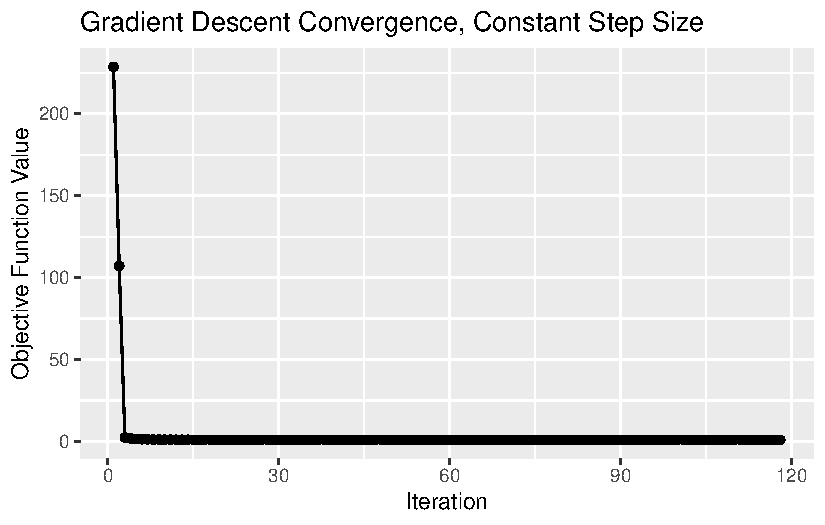
\includegraphics{506021334_Stats102B_hw_1_files/figure-pdf/unnamed-chunk-1-1.pdf}

\begin{Shaded}
\begin{Highlighting}[]
\FunctionTok{ggplot}\NormalTok{(f\_k\_backtrack, }\FunctionTok{aes}\NormalTok{(}\AttributeTok{x=}\NormalTok{iterations, }\AttributeTok{y=}\NormalTok{obj\_values)) }\SpecialCharTok{+} 
  \FunctionTok{geom\_point}\NormalTok{() }\SpecialCharTok{+} 
  \FunctionTok{geom\_line}\NormalTok{() }\SpecialCharTok{+} 
  \FunctionTok{ggtitle}\NormalTok{(}\StringTok{"Gradient Descent Convergence, Backtracking Line Search"}\NormalTok{) }\SpecialCharTok{+} 
  \FunctionTok{xlab}\NormalTok{(}\StringTok{"Iteration"}\NormalTok{) }\SpecialCharTok{+} \FunctionTok{ylab}\NormalTok{(}\StringTok{"Objective Function Value"}\NormalTok{)}
\end{Highlighting}
\end{Shaded}

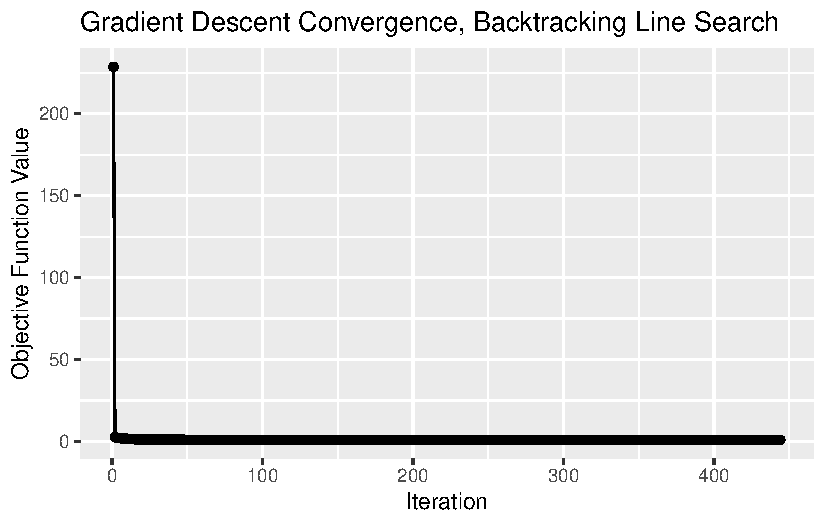
\includegraphics{506021334_Stats102B_hw_1_files/figure-pdf/unnamed-chunk-1-2.pdf}

\subsubsection{\texorpdfstring{3) For the the gradient descent method
with backtracking line search, plot the step size \(η_k\) selected at
step k as a function of k. Comment on the
result}{3) For the the gradient descent method with backtracking line search, plot the step size η\_k selected at step k as a function of k. Comment on the result}}\label{for-the-the-gradient-descent-method-with-backtracking-line-search-plot-the-step-size-ux3b7_k-selected-at-step-k-as-a-function-of-k.-comment-on-the-result}

\begin{Shaded}
\begin{Highlighting}[]
\NormalTok{iterations }\OtherTok{\textless{}{-}} \DecValTok{1}\SpecialCharTok{:}\NormalTok{minimize\_backtrack}\SpecialCharTok{$}\NormalTok{last\_iter}
\NormalTok{eta\_values }\OtherTok{\textless{}{-}}\NormalTok{ minimize\_backtrack}\SpecialCharTok{$}\NormalTok{eta\_values[iterations]}
\NormalTok{eta\_backtrack }\OtherTok{\textless{}{-}} \FunctionTok{cbind}\NormalTok{(eta\_values, iterations)}

\FunctionTok{ggplot}\NormalTok{(eta\_backtrack, }\FunctionTok{aes}\NormalTok{(}\AttributeTok{x=}\NormalTok{iterations, }\AttributeTok{y=}\NormalTok{eta\_values)) }\SpecialCharTok{+} 
  \FunctionTok{geom\_point}\NormalTok{() }\SpecialCharTok{+} 
  \FunctionTok{geom\_line}\NormalTok{() }\SpecialCharTok{+} 
  \FunctionTok{ggtitle}\NormalTok{(}\StringTok{"Gradient Descent Eta Values, BLS"}\NormalTok{) }\SpecialCharTok{+} 
  \FunctionTok{xlab}\NormalTok{(}\StringTok{"Iteration"}\NormalTok{) }\SpecialCharTok{+} \FunctionTok{ylab}\NormalTok{(}\StringTok{"Eta Value"}\NormalTok{)}
\end{Highlighting}
\end{Shaded}

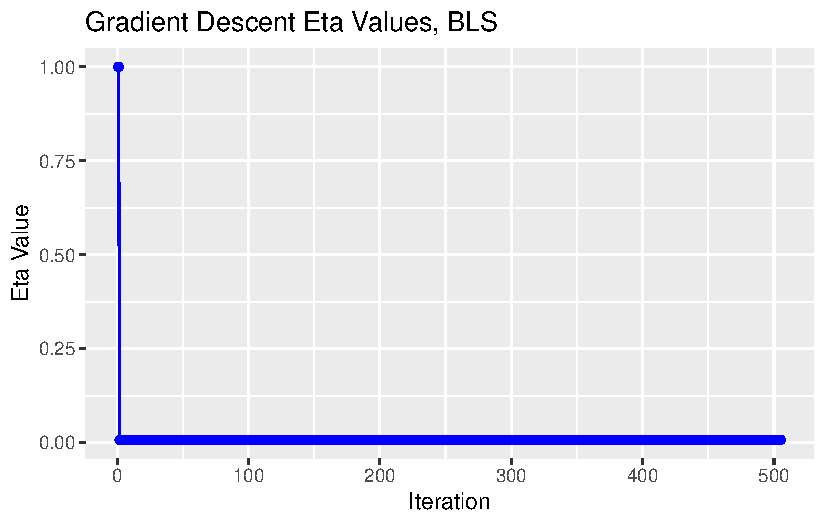
\includegraphics{506021334_Stats102B_hw_1_files/figure-pdf/unnamed-chunk-2-1.pdf}

We can see that the step size was initially 0.02, but at the very first
few iterations the Armijo condition immediately reduced the step size to
a very small number \textless{} 0.005 in order to prevent overshooting.
This condition held for the rest of the iterations until the algorithm
converged eventually, after around 443 iterations. Compared to the
constant step size gradient descent, the step size was much smaller for
all the iterations, meaning that it converged with \textgreater{} 300
more iterations than the constant step size gradient descent. Although
using a large step size like 0.02 would be much faster, it seems like
the step sizes were chosen to be a safer bound so that the algorithm
would not overshoot

\section{Problem 2}\label{problem-2}




\end{document}
